%% -*- coding:utf-8 -*-

\chapter{Tree Adjoining Grammar}
\label{Kapitel-TAG}

\newcommand{\dotted}[0]{\makedash{2pt}}
\newcommand{\g}[1]{{\footnotesize $#1$}}


\emph{Tree Adjoining Grammar} (TAG)\is{Tree Adjoining Grammar (TAG)|(}
was developed by Aravind Joshi at the University of Pennsylvania in the USA \citep*{JLT75a-u}. 
Several important dissertations in TAG have been supervised by Aravind
Joshi and Anthony Kroch at the University of Pennsylvania (\eg \citealp{Rambow94a}).
Other research centers with a focus on TAG are Paris~7 (Anne Abeill\'{e}), Columbia University in the USA
(Owen Rambow) and Düsseldorf, Germany (Laura Kallmeyer).
\citew{Rambow94a} and \citew{Gerdes2002b-u} are more detailed studies of German.\footnote{%
	Since my knowledge of French leaves something to be desired, I just refer to the literature in French here without being
	able to comment on the content.%
}
%Viola: \todostefan{leaves a little oder much - something wie als nettes Understatement im Deutschen passt hier leider nicht :-)}

%\largerpage[4]
TAG and its variants with relevant extensions are of interest because it is assumed that this grammatical formalism can -- with regard to its
expressive power -- relatively accurately represent what humans do when they produce or comprehend natural language.
The expressive power of Generalized Phrase Structure Grammar\indexgpsg was deliberately constrained so that it corresponds to context"=free
phrase structure grammars\is{context"=free grammar} (Type-2 languages) and it has in fact been demonstrated that this is not enough \citep{Shieber85a,Culy85a}.\footnote{%
	See \citet{Pullum86a} for a historical overview of the complexity debate and G.\ \citew{GMueller2011a} for argumentation for the non"=context"=free nature
	of German, which follows parallel to  Culy with regard to the N-P-N construction\is{construction!N-P-N} (see Section~\ref{Abschnitt-NPN-Konstruktion}).%
	} Grammatical theories such as HPSG\indexhpsg and CxG\indexcxg can generate/describe so"=called Type-0 languages and are thereby far above the level
	of complexity presently assumed for natural languages. 
The assumption is that this complexity lies somewhere between context"=free\is{complexity class}\is{context"=free grammar}
and context"=sensitive\is{context"=sensitive grammar} (Type-1) languages. This class is thus referred to as \emph{mildly context"=sensitive}\is{mildly context"=sensitive grammar!context"=sensitive grammar}.
Certain TAG"=variants are inside of this language class and it is assumed that they can produce exactly those structures that occur in
natural languages. For more on complexity, see Section~\ref{Abschnitt-Kompetenz-Performanz-TAG} and Chapter~\ref{sec-generative-capacity}.

There are various systems for the processing of TAG grammars \citep*{DHSSX2000a-u,PKMLD2008a-u,KLMPDE2008a-u,Koller2017a-u}.
Smaller and larger TAG fragments have been developed for the following languages:
\begin{itemize}
\item Arabic\il{Arabic} \citep*{ArabTAG2008a},
\item German \citep{Rambow94a,Gerdes2002a,KY2004b,Lichte2007a},
\item English\il{English} \citep{XTAG2001a,Frank2002a-u,KrochJoshi87a-u},
\item French\il{French} \citep{Abeille88a,Candito96a,Candito98a,Candito99a-u,Crabbe2005a-u},
\item Italian\il{Italian} \citep{Candito98a,Candito99a-u},%,Kinyon2003a}
\item Korean\il{Korean} \citep*{HYKP2000a-u,KY2004b},
\item Vietnamese\il{Vietnamese} \citep*{VietnameseTAG2008a}
%\item Tagalog\il{Tagalog} \citep{MR2003a}
\end{itemize}
\citet{Candito96a} has developed a system for the representation of meta grammars which allows the
uniform specification of crosslinguistic generalizations. This system was used by some of the
projects mentioned above for the derivation of grammars for specific languages. For instance
\citet*{KSYJ2006a} derive the verb second languages from a common meta grammar. Among those grammars for verb second
languages is a grammar of Yiddish\il{Yiddish} for which there was no TAG grammar until 2006.

\citet{Resnik92a} combines TAG with a statistics\is{statistics} component.


\section{General remarks on representational format}
\label{sec-tag-allgemein}

\subsection{Representation of valence information}

Figure~\vref{abb-elementare-Baeume}\is{valence|(} shows so"=called elementary trees\is{elementary tree}.
These are present in the lexicon and can be combined to create larger trees.
\begin{figure}
\hfill
\begin{forest}
tag
[NP
	[John]]
\end{forest}
\hfill
\begin{forest}
tag
[S
	[NP$\downarrow$]
	[VP
		[V
			[laughs]]]]
\end{forest}
\hfill
\begin{forest}
tag
[VP
	[ADV
		[always]]
	[VP*]]
\end{forest}
\hfill\mbox{}
\caption{\label{abb-elementare-Baeume}Elementary trees}
\end{figure}%
%
Nodes for the insertion of arguments are specially marked (NP$\downarrow$\is{$\downarrow$} in the tree for \emph{laughs}).
Nodes for the insertion of adjuncts\is{adjunct} into a tree are also marked (VP$^*$\is{*} in the tree for \emph{always}).
Grammars where elementary trees always contain at least one word are referred to as
\emph{Lexicalized Tree Adjoining Grammar} (LTAG, \citew*{SAJ88a-u}).\is{valence|)} 

\subsection{Substitution}

%\largerpage[2]
Figure~\vref{abb-Substitution}\is{substitution|(} shows the substitution of nodes.
\begin{figure}
\centerline{%
\begin{forest}
tag
[S
	[NP$\downarrow$,
          [NP, substitution
            [John]]]
	[VP
		[V
			[laughs]]]]
\end{forest}
\hspace{1em}
$\leadsto$
\hspace{1em}
\begin{forest}
tag
[S
	[NP
		[John]]
	[VP
		[V
			[laughs]]]]
\end{forest}
}
\caption{\label{abb-Substitution}Substitution}
\end{figure}%
Other subtrees have to be inserted into substitution nodes such as the NP node in the tree for \emph{laughs}.
The tree for \emph{John} is inserted there in the example derivation.\is{substitution|)}

\subsection{Adjunction}

Figure~\vref{abb-Adjunktion}\is{adjunction|(}\is{adjunct|(} shows an example of how the adjunction tree for \emph{always} can be used. 

%
\begin{figure}
\centerline{%
\begin{forest}
tag
[S
	[NP
		[John]]
	[VP
		[V
			[laughs]]]]
\end{forest}
\hspace{0.5cm}
\begin{forest}
tag
[VP
	[ADV
		[always]]
	[VP*]]
\end{forest}
\hspace{1em}
$\leadsto$
\hspace{1em}
\begin{forest}
tag
[S
	[NP
		[John]]
	[VP
		[ADV
			[always]]
		[VP
			[V
				[laughs]]]]]
\end{forest}
}
\caption{\label{abb-Adjunktion}Adjunction}
\end{figure}%
Adjunction trees can be inserted into other trees. Upon insertion, the target node (bearing  the
same category as the node marked with `*') is replaced by the adjunction tree.
\is{adjunction|)}\is{adjunct|)}

\largerpage[-1]
TAG differs considerably from the simple phrase structure grammars we encountered in
Chapter~\ref{Kapitel-PSG} in that the trees extend over a larger domain: for example, there is an NP
node in the tree for \emph{laughs} that is not a sister of the verb. In a phrase structure grammar (and of course in GB\indexgb and GPSG\indexgpsg since
these theories are more or less directly built on phrase structure grammars), it is only ever possible to describe subtrees with a depth of one level.
For the tree for \emph{laughs}, the relevant rules would be those in (\mex{1}):
\ea
\begin{tabular}[t]{@{}l@{ }l}
S  & $\to$ NP VP\\
VP & $\to$ V\\
V  & $\to$ laughs\\
\end{tabular}
\z
In this context, it is common to speak of \emph{locality domains}\is{locality}. The extension of the
locality domain is of particular importance for the analysis of idioms (see Section~\ref{Abschnitt-Diskussion-Lokalitaet}).

TAG differs from other grammatical theories in that it is possible for structures to be broken up again.
In this way, it is possible to use adjunction to insert any amount of material into a given tree and thereby cause originally adjacent constituents
to end up being arbitrarily far away from each other in the final tree. As we will see in Section~\ref{TAG-Fernabh}, this property is important for the
analysis of long"=distance dependencies without movement.

\subsection{Semantics}

There are different approaches to the syntax"=semantics interface in TAG.
One possibility is to assign a semantic representation to every node in the tree. The alternative is to assign each elementary tree
exactly one semantic representation. The semantics construction does not make reference to syntactic structure but rather the way
the structure is combined. This kind of approach has been proposed by \citet{CK98a} and then by \citet{KJ2003a}, who build on it.
The basic mechanisms will be briefly presented in what follows.

%\begin{sloppypar}
In the literature on TAG, a distinction is made between derived trees and derivation trees\is{derivation tree}.
Derived trees correspond to constituent structure (the trees for \emph{John laughs} and
\emph{John always laughs} in Figures~\ref{abb-Substitution} and ~\ref{abb-Adjunktion}).
The derivation tree contains the derivational history, that is, information about how the elementary trees were combined.
The elements in a derivation tree represent predicate"=argument dependencies, which is why it is possible to derive
a semantic derivation tree from them. This will be shown on the basis of the sentence in (\mex{1}):
%\end{sloppypar}

\ea
Max likes Anouk.
\z
The elementary tree for (\mex{0}) and the derived tree are given in Figure~\vref{Abbildung-Max-likes-Anouk}.
\begin{figure}
\centering
\begin{forest}
tag
[S
	[NP$\downarrow$
          [NP,substitution [Max]]]
	[VP
		[V
			[likes]]
		[NP$\downarrow$
                  [NP,substitution [Anouk] ]]]]
\end{forest}
\hspace{1em}
$\leadsto$
\hspace{1em}
\begin{forest}
tag
[S
	[NP
		[Max]]
	[VP
		[V
			[likes]]
		[NP
			[Anouk]]]]
\end{forest}
\caption{\label{Abbildung-Max-likes-Anouk}Elementary trees and derived tree for \emph{Max likes Anouk.}}
\end{figure}%
The nodes in trees are numbered from top to bottom and from left to right. The result of this numbering of nodes for \emph{likes} 
is shown in Figure~\vref{Abbildung-Knotenpositionen}. The topmost node in the tree for  \emph{likes} is S and has the position 0.
Beneath S, there is an NP and a VP node. These nodes are again numbered starting at
1. NP has the position 1 and VP the position 2.
The VP node has in turn two daughters: V and the object NP. V receives number 1 and the object NP 2. This makes it possible to combine these numbers and then it is possible to unambiguously access individual elements in the tree. The position for the subject NP
is 1 since this is a daughter of S and occurs in first position. The object NP has the numeric
sequence 2.2 since it is below the VP (the second daughter of S = 2) and occurs in second position (the second daughter of VP = 2).

\begin{figure}
\centerline{%
\begin{forest}
tag
[S {(0)}
	[NP$\downarrow$ {(1)}]
	[VP {(2)}
		[V {(2.1)}
			[likes]]
		[NP$\downarrow$ {(2.2)}]]]
\end{forest}
}
\caption{\label{Abbildung-Knotenpositionen}Node positions in the elementary tree for \emph{likes}}
\end{figure}%

With these tree positions, the derivation tree for (\mex{0}) can be represented as in Figure~\vref{Abbildung-Ableitungsbaum}.
\begin{figure}
\centerline{%
\begin{forest}
[likes, l sep+=1em
	[Max,edge label={node[midway,left]{1~~}}]
	[Anouk,edge label={node[midway,right]{~2.2}}]]
\end{forest}
}
\caption{\label{Abbildung-Ableitungsbaum}Derivation tree for \emph{Max likes Anouk.}}
\end{figure}%
The derivation tree expresses the fact that the elementary tree for \emph{likes} was combined with two arguments that were inserted
into the substitution positions 1 and 2.2. The derivation tree also contains information about what exactly was placed into these
nodes.

\citet{KJ2003a} use a variant of \emph{Minimal Recursion
Semantics}\indexmrs as their semantic representational formalism
\citep*{CFPS2005a}. I will use a considerably simplified representation here, as I did in
Section~\ref{Abschnitt-HPSG-Semantik} on semantics in HPSG. For the elementary trees \emph{Max},
\emph{likes} and \emph{Anouk}, we can assume the semantic representations in (\mex{1}). 
\ea
Semantic representations for elementary trees:\\*
\begin{tabular}[t]{|l|}\hline
max(x)\\\hline
arg: $-$\\\hline
\end{tabular}
\hfill
\begin{tabular}[t]{|l|}\hline
like(x$_1$, x$_2$)\\\hline
arg: \sliste{ x$_1$, 1 }, \sliste{ x$_2$, 2.2 }\\\hline
\end{tabular}
\hfill
\begin{tabular}[t]{|l|}\hline
anouk(y)\\\hline
arg: $-$\\\hline
\end{tabular}
\hfill\mbox{}
\z
In a substitution operation, a variable is assigned a value. If, for example, the elementary tree for \emph{Max}
is inserted into the subject position of the tree for \emph{likes}, then x$_1$ is identified with x.
In the same way, x$_2$ is identified with y if the tree for \emph{Anouk} is inserted into the object position.
The result of these combinations is the representation in 
(\mex{1}):
\eas
Combination of the meaning of elementary trees:\\
\begin{tabular}[t]{|l|}\hline
like(x, y)\\
max(x)\\
anouk(y)\\\hline
arg: $-$\\\hline
\end{tabular}
\zs

\noindent
\citet{KJ2003a} show how an extension of TAG, Multi-Component LTAG\is{Multi-Component TAG}, can handle quantifier scope\is{scope} and discuss complex
cases with embedded verbs. Interested readers are referred to the original article.

\section{Local reordering}
\label{Abschnitt-MC-TAG}\label{sec-ld-lp-tag}

%\addlines
In\is{constituent order|(} TAG, there is a family of trees for each word. In order to account for ordering variants, one can assume that there
are six trees corresponding to a ditransitive verb and that each of these corresponds to a different ordering of the arguments.
Trees are connected to one another via lexical rules\is{lexical rule}. This lexical rule"=based
analysis is parallel to the one developed by \citet{Uszkoreit86b} in Categorial Grammar. 

Alternatively, one could assume a format for TAG structures similar to what we referred to as the
ID/LP format\is{ID/LP grammar} in the chapter
on GPSG. \citet{Joshi87b} defines an elementary structure as a pair that consists of a dominance structure and linearization constraints.
Unlike GPSG, linearization rules do not hold for all dominance rules but rather for a particular dominance structure. This is parallel to what
we saw in Section~\ref{sec-ECG} on Embodied-CxG. Figure~\vref{Abbildung-TAG-S} shows a dominance tree with numbered nodes.
\begin{figure}
\centerline{%
$\alpha$ = \begin{forest}
baseline, tag
[S$_0$
	[NP$_1$]
	[VP$_2$
		[V$_{2.1}$]
		[NP$_{2.2}$]]]
\end{forest}
}
\caption{\label{Abbildung-TAG-S}Dominance structure with numbered nodes}
\end{figure}%
If we combine this dominance structure with the linearization rules in (\mex{1}), we arrive at the exact order that we would get with
ordinary phrase structure rules, namely NP$_1$ V NP$_2$.
\ea
LP$^\alpha_1$ = \{ 1 $<$ 2, 2.1 $<$ 2.2 \}
\z
If one specifies the linearization restrictions as in (\mex{1}), all the orders in (\mex{2}) are permitted, since the empty set means that we do not state any restrictions at all.
\ea
LP$^\alpha_2$ = \{ \}
\z
\eal
\ex NP$_1$ V NP$_2$
\ex NP$_2$ V NP$_1$
\ex NP$_1$ NP$_2$ V 
\ex NP$_2$ NP$_1$ V
\ex V NP$_1$ NP$_2$
\ex V NP$_2$ NP$_1$ 
\zl
This means that it is possible to derive all orders that were derived in GPSG\indexgpsg with flat sentence rules despite the fact that there is
a constituent in the tree that consists of NP and VP. Since the dominance rules include a larger
locality domain, such grammars are called LD/LP grammars (local dominance/linear precedence) rather
than ID/LP grammars (immediate dominance/linear precedence) \citep*{JSW90a-u}.

Simple variants of TAG such as those presented in Section~\ref{sec-tag-allgemein} cannot deal with reordering if the arguments of different verbs
are scrambled as in (\mex{1}).
\ea
\label{ex-weil-ihm-das-Buch-jemand-zu-lesen-versprochen-hat-drei}
\gll weil    ihm das Buch jemand   zu lesen versprochen hat\footnotemark\\
     because him.\dat{} the.\acc{} book somebody.\nom{} to read promised has\\
\footnotetext{%
For more on this kind of examples, see \citew{Bech55a}.
}
\glt `because somebody promised him to read the book'
\z
In (\mex{0}), \emph{das Buch} `the book' is the object of \emph{zu lesen} `to read', and \emph{ihm}
`him' and \emph{jemand} `somebody' are dependent on \emph{versprochen} and \emph{hat}, respectively.
These cases can be analyzed by LD/LP"=TAG developed by \citet{Joshi87b} and Free Order TAG
(FO"=TAG\is{TAG!Free Order (FO"=TAG)}) \citep*[\page 21]{BJR91a} since both of these TAG variants allow for
crossing edges.\is{projectivity}

Since certain restrictions cannot be expressed in FO"=TAG \citep[\page 48--50]{Rambow94a}, so"=called Multi"=Component TAG\is{Multi-Component TAG}\is{Tree Adjoining Grammar (TAG)!Multi"=Component (MC-TAG)|(} was developed.
\citet*{JBR2000a} illustrate the problem that simple LTAG grammars have with sentences such as (\mex{0}) using examples such as (\mex{1}):\footnote{%
  The authors use \emph{versprochen hat} `has promised' rather than \emph{versprach} `promised', which sounds better but does not correspond
  to the trees they use.
}
\eal
\ex 
\gll \ldots{} daß  der        Detektiv  dem        Klienten [den Verdächtigen des Verbrechens zu überführen] versprach\\
         {}   that the.\nom{} detective the.\dat{} client   \spacebr{}the.\acc{} suspect the.\gen{} crime to indict promised\\
  \glt `that the detective promised the client to indict the suspect of the crime'
\ex\label{Beispiel-Joshi-NP4} 
\gll \ldots{} daß  des        Verbrechens$_k$ der        Detektiv  den Verdächtigen$_j$~~~~~~~~~ dem         Klienten [\_$_j$ \_$_k$ zu überführen] versprach\\
      {}      that the.\gen{} crime           the.\nom{} detective the.\acc{} suspect   the.\dat{}  client   {}      {}     to indict      promised\\
\zl
\largerpage
In LTAG, the elementary trees for the relevant verbs look as shown in Figure~\vref{Abbildung-Kontrollverben-TAG}.
\begin{figure}
\oneline{%
\begin{forest}
tag, baseline
[S
	[NP$_2^2\downarrow$]
	[S
		[NP$_2^1\downarrow$]
		[S
			[NP
				[PRO]]
			[VP
				[NP$_2^1$
					[e]]
				[NP$_2^2$
					[e]]
				[V$_2$
					[zu überführen;to indict]]]]]]
\end{forest}
\begin{forest}
tag, baseline
[S
	[NP$_1^1\downarrow$]
	[VP
		[NP$_1^2\downarrow$]
		[S*]
		[V$_1$
		[versprach;promised]]]]
\end{forest}
}
\caption{\label{Abbildung-Kontrollverben-TAG}Elementary trees of an infinitive and a control verb} 
\end{figure}%
The verbs are numbered according to their level of embedding. The NP arguments of a verb bear the same index as that verb
and each has a superscript number that distinguishes it from the other arguments.
The trees are very similar to those in GB\indexgb. In particular, it is assumed that the subject occurs outside the VP.
For non"=finite verbs, it is assumed that the subject is realized by PRO\is{PRO}. PRO is, like \emph{e}, a phonologically empty pronominal
category\is{empty element!PRO|see{PRO}} that also comes from GB.
The left tree in Figure~\ref{Abbildung-Kontrollverben-TAG} contains traces in the normal position of the arguments and the relevant
NP slots in higher trees positions. An interesting difference to other theories is that these traces\is{empty element} only exist in the tree. They are not
represented as individual entries in the lexicon as the lexicon only contains words and the corresponding trees.

%\largerpage
The tree for \emph{versprach} `promised' can be inserted into any S node in the tree for \emph{zu überführen} `to indict' and results in
trees such as those in the Figures~\ref{Abbildung-TAG-Permutation-one} and~\ref{Abbildung-TAG-Permutation-two}.
%\thefiguresref{Abbildung-TAG-Permutation-one}{Abbildung-TAG-Permutation-two}.
\begin{figure}
\centerline{%
\begin{forest}
tag
[S
	[NP$_2^2\downarrow$]
	[S
		[NP$_2^1\downarrow$]
		[\textit{S}
			[NP$_1^1\downarrow$]
			[VP
				[NP$_1^2\downarrow$]
				[\textit{S}
					[NP
						[PRO]]
					[VP
						[NP$_2^1$
							[e]]
						[NP$_2^2$
							[e]]
						[V$_2$
							[zu überführen;to indict]]]]
				[V$_1$
					[versprach;promised]]]]]]
\end{forest}
}
\caption{Analysis of the order NP$_2^2$ NP$_2^1$ NP$_1^1$ NP$_1^2$ V$_{2}$V$_{1}$: adjunction to the lowest S node}\label{Abbildung-TAG-Permutation-one}
\end{figure}%
%
\begin{figure}
\centerline{%
\begin{forest}
tag
[S
	[NP$_2^2\downarrow$]
	[\textit{S}
		[NP$_1^1\downarrow$]
		[VP
			[NP$_1^2\downarrow$]
			[\textit{S}
				[NP$_2^1\downarrow$]
				[S
					[NP
						[PRO]]
					[VP
						[NP$_2^1$
							[e]]
						[NP$_2^2$
							[e]]
						[V$_2$
							[zu überführen;to indict]]]]]
			[V$_1$
				[versprach;promised]]]]]
\end{forest}
}
\caption{Analysis of the order NP$_2^2$ NP$_1^1$ NP$_1^2$ NP$_2^1$ V$_{2}$V$_{1}$: adjunction to the S node between NP$_2^2$ and NP$_2^1$}\label{Abbildung-TAG-Permutation-two}
\end{figure}%

\noindent
In Figure~\ref{Abbildung-TAG-Permutation-one}, the tree for \emph{versprach} is inserted directly above the PRO NP and in Figure~\ref{Abbildung-TAG-Permutation-two} above
NP$_2^1$.

\largerpage
It is clear that it is not possible to derive a tree in this way where an argument of \emph{überführen} `to indict' occurs between the arguments of \emph{versprach}
`promised'. \citet*{JBR2000a} therefore suggest an extension of the LTAG formalism. In MC-TAG, the grammar does not consist of elementary trees but rather
finite sets of elementary trees. In every derivational step, a set is selected and the elements of that set are simultaneously added to the tree.
Figure~\vref{Abbildung-MC-TAG-versprach} shows an elementary tree for \emph{versprach} `promised' consisting of multiple components.
\begin{figure}
%% ~\\[2ex]
%% \centerline{%
%% \menge{
%% \forestset{begin draw/.code={\begin{tikzpicture}[baseline=(current bounding box.center)]}}
%% \hspace{2ex}
%% \begin{forest}
%% [S
%% 	[NP$_1^1\downarrow$]
%% 	[\subnode{s1}{S} ]]
%% \end{forest}
%% \hspace{1.5cm}
%% \begin{forest}
%% [\subnode{s2}{S}
%% 	[NP$_1^1$
%% 		[e]]
%% 	[VP
%% 		[NP$_1^2\downarrow$]
%% 		[S*]
%% 		[V$_1$
%% 			[versprach]]]]
%% \end{forest}
%% \hspace{2ex}
%% \begin{tikzpicture}[overlay,remember picture,out=-70,in=110,dashed]
%% \draw (s1) to (s2);
%% \end{tikzpicture}
%% }
%% }
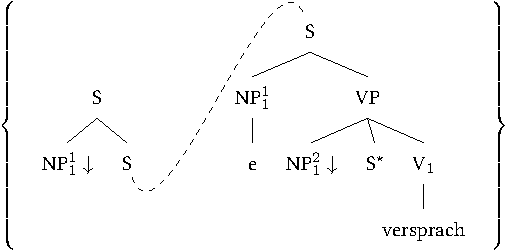
\includegraphics{Figures/tag-versprach-lsp-crop}
\caption{\label{Abbildung-MC-TAG-versprach}Elementary tree set for \emph{versprach} consisting of multiple components}
\end{figure}%
This tree contains a trace of NP$_1^1$ that was moved to the left. The bottom"=left S node and the top"=right S node are connected by a dashed line
that indicates the dominance relation. However, immediate dominance is not required. Therefore, it is possible to insert the two subtrees into another tree
separately from each other and thereby analyze the order in Figure~\vref{Abbildung-TAG-Permutation3}, for example.\is{Multi-Component TAG}\is{Tree Adjoining Grammar (TAG)!Multi"=Component (MC-TAG)|)} 
\begin{figure}
\centerline{%
\begin{forest}
tag
[S
	[NP$_1^1\downarrow$]
	[S
		[NP$_2^2\downarrow$]
		[S
			[NP$_1^1$
				[e]]
			[VP
				[NP$_1^2\downarrow$]
				[S
					[NP$_2^1\downarrow$]
					[S
						[NP
							[PRO]]
						[VP
							[NP$_2^1$
								[e]]
							[NP$_2^2$
								[e]]
							[V$_2$
								[zu überführen;to indict]]]]]
				[V$_1$
					[versprach;promised]]]]]]
\end{forest}
}
\caption{\label{Abbildung-TAG-Permutation3}Analysis of the order NP$_1^1$ NP$_2^2$ NP$_1^2$ NP$_2^1$ V$_{2}$V$_{1}$: adjunction to the S node between NP$_2^2$ and NP$_2^1$}
\end{figure}%

%Andere Varianten, die andere Konstituentenanordnungen zulassen sind V-TAG\is{Tree Adjoining Grammar@\emph{Tree Adjoining Grammar} (TAG)!\emph{Vektor} (V-TAG)} \citep{Rambow94a} und TT-MC-TAG\is{Tree Adjoining Grammar@\emph{Tree Adjoining Grammar} (TAG)!\emph{Tree Tuple MC-TAG} (TT-MC-TAG)} \citep{Lichte2007a}.\is{Konstituentenstellung|)}
Other variants of TAG that allow for other constituent orders are V-TAG\is{Tree Adjoining Grammar (TAG)!Vector (V-TAG)} \citep{Rambow94a} 
and TT-MC-TAG\is{Tree Adjoining Grammar (TAG)!Tree Tuple MC-TAG (TT-MC-TAG)} \citep{Lichte2007a}.\is{constituent order|)}

\section{Verb position}

\largerpage
The position of the verb\is{verb position|(} can be analyzed in a parallel way to the GPSG analysis:
the verb can be realized in initial or in final position in a given linearization domain. Since the
verb position has an effect on the clause type and hence on semantics, a lexical rule"=based
analysis would be also viable: a tree with the finite verb in initial position is licensed by a
lexical rule that takes a tree with the verb in final position as input. This would be similar to
the analyses in GB, Minimalism, and HPSG.
\is{verb position|)}

\section{Passive}

There is\is{passive|(} a possible analysis for the passive that is analogous to the transformations in Transformational Grammar: one assumes lexical rules that
license a lexical item with a passive tree for every lexical item with an active tree \citep[\page 50--51]{KJ85a}. 

\citet[\page 55]{KJ85a} propose an alternative to this transformation"=like approach that more adequately handles so"=called raising constructions\is{raising}.
Their analysis assumes that arguments of verbs are represented in subcategorization lists. Verbs are entered into trees that match their subcategorization
list. Kroch and Joshi formulate a lexical rule that corresponds to the HPSG lexical rule that was discussed on page~\pageref{pass-lr-mlr}, that is,
an accusative object is explicitly mentioned in the input of the lexical rule. Kroch and Joshi then suggest a complex analysis of the impersonal passive which
uses a semantic null role for a non-realized object of intransitive verbs (p.\,56). Such an analysis
with abstract auxiliary entities can be avoided easily: one can instead use the HPSG\indexhpsg
analysis going back to \citet{Haider86}, which was presented in Section~\ref{Abschnitt-HPSG-Passiv}.
%\largerpage

There\is{inheritance!multiple|(} are also proposals in TAG that use inheritance to deal with valence changing processes 
in general and the passive in particular (\citealp{Candito96a} and \citealp*{KSYJ2006a} following Candito). As we saw in Section~\ref{Abschnitt-Passiv-CxG} of 
the Chapter on Construction Grammar, inheritance is not a suitable descriptive tool for valence changing processes. This is because these kinds of processes
interact syntactically and semantically in a number of ways and can also be applied multiple times
(\citealp{Mueller2006d,Mueller2007d}; \citeyear[Section~7.5.2]{MuellerLehrbuch1};
\citeyear{MuellerUnifying}; \citeyear{MWArgSt}). See also Section~\ref{relations-sec} of this book.%
\is{inheritance!multiple|)}\is{passive|)}

\section{Long"=distance dependencies}
\label{TAG-Fernabh}

The\il{English|(}\is{long"=distance dependency|(} analysis of long"=distance dependencies in TAG is handled with the standard apparatus: simple trees are inserted
into the middle of other trees. Figure~\vref{abb-nld-TAG} shows an example of the analysis of (\mex{1}):
\ea
Who$_i$ did John tell Sam that Bill likes \_$_i$?
\z
%
\begin{figure}
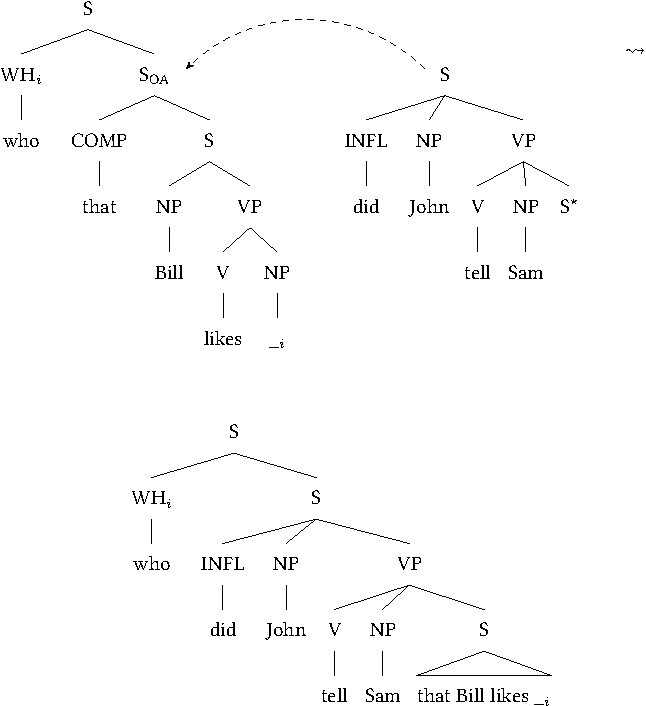
\includegraphics{Figures/tag-long-distance-dependencies-crop}
%%
%% Does not work with texlive 2015
%% %\oneline{%
%% \centerline{%
%% \begin{forest}
%% tag
%% [S
%% 	[WH$_i$
%% 		[who]]
%% 	[\tikzmark{soa}{S\sub{OA}}
%% 		[COMP
%% 			[that]]
%% 		[S
%% 			[NP
%% 				[Bill]]
%% 			[VP
%% 				[V
%% 					[likes]]
%% 				[NP
%% 					[\noexpand\_$_i$]]]]]]
%% \end{forest}
%% \hspace{0.5cm}
%% \begin{forest}
%% tag
%% [\tikzmark{s}{S}
%% 	[INFL
%% 		[did]]
%% 	[NP
%% 		[John]]
%% 	[VP
%% 		[V
%% 			[tell]]
%% 		[NP
%% 			[Sam]]
%% 		[S*]]]
%% \end{forest}
%% \qquad \raisebox{2cm}{$\rightsquigarrow$} \qquad
%% }\vspace{2\baselineskip}
%% \begin{forest}
%% tag
%% [S
%% 	[WH$_i$
%% 		[who]]
%% 	[S
%% 		[INFL
%% 			[did]]
%% 		[NP
%% 			[John]]
%% 		[VP
%% 			[V
%% 				[tell]]
%% 			[NP
%% 				[Sam]]
%% 			[S
%% 				[that Bill likes \noexpand\_$_i$, roof]]]]]
%% \end{forest}
%% \begin{tikzpicture}[overlay,remember picture]
%% \draw[->, dashed, bend angle=45, bend right] ($(pic cs:s)+(-0.25,0.2)$) to($(pic cs:soa)+(0.8,.2)$);
%%
%% \end{tikzpicture}
%%
%% {%\dotted
%% % todo \anodecurve[l]{s4}[tr]{s2}{0.1in}[3ex]%
%% }
%% \hspace{1ex}
%% $\leadsto$
%}
\caption{\label{abb-nld-TAG}Analysis of long"=distance dependencies in TAG}
\end{figure}%
The tree for \emph{WH COMP NP likes \_$_i$} belongs to the tree family of \emph{likes} and is therefore
present in the lexicon.
The tree for \emph{tell} is adjoined to this tree, that is, this tree is inserted in the middle of the tree for
\emph{who that Bill likes \_$_i$}. Such an insertion operation can be applied multiple times so that sentences such as (\mex{1})
where \emph{who} is moved across multiple sentence boundaries can be analyzed:
\ea 
Who$_i$ did John tell Sam that Mary said that Bill likes \_$_i$?
\z
%
There is another important detail: although the tree for (\mex{1}) has the category S, (\mex{1}) is not a grammatical
sentence of English.
\ea[*]{
who that Bill likes
}
\z
This has to be captured somehow. In TAG, the marking OA ensures that a tree counts as incomplete. If
a tree contains a node with marking OA, then an obligatory adjunction\is{adjunction!obligatory}
operation must take place at the relevant position.\il{English|)}\is{long"=distance dependency|)} 

\section{New developments and theoretical variants}

In Section~\ref{Abschnitt-MC-TAG}, we introduced Multi"=Component"=TAG. There are a large number of TAG variants with different formal properties.
\citet[\page
]{Rambow94a} gives an overview of the variants existing in 1994. In the following, I will discuss
two interesting variants of TAG: Feature Structure"=Based TAG (FTAG\indexftag, \citealp{VSJ88a}) and
Vector"=TAG (V"=TAG, \citealp{Rambow94a}). 

\subsection{FTAG}

In FTAG\is{Tree Adjoining Grammar (TAG)!Feature Structure"=Based (FTAG)|(}, nodes are not atomic (N,
NP, VP or S), but instead consist of feature descriptions. With the exception of substitution nodes, each node has a top structure and a bottom structure.
The top structure says something about what kind of properties a given tree has inside a larger structure, and the bottom structure says something
about the properties of the structure below the node.
Substitution nodes only have a top structure. Figure~\vref{Abbildung-FTAG-laughs} shows an example
tree for \emph{laughs}.\todostefan{geschwungenen Pfeil, alignierte Knoten}
\begin{figure}
\centerline{%
\begin{forest}
tag
[{\ms{
   cat & {\upshape S}\\
 }\\
\ms{
   cat & {\upshape S}
}}
  [\ms{
    cat & {\upshape NP}\\
    agr & \ibox{1}\\
   }
%
   [{[~]\\
    \ms{
       cat & {\upshape NP}\\
       agr & \ms{
              per & 3\\ 
              num & sing\\
             }\\
      }}, substitution,tier=2
      [John, tier=word] ] ]
  [{\ms{
     cat & {\upshape VP}\\
     agr & \ibox{1} \ms{
                    per & 3\\ 
                    num & sing\\
                    }\\
     }\\
     \ms{ 
     cat & {\upshape VP}\\
     }}
     [{\ms{
          cat & {\upshape V}\\
         }\\
       \ms{
          cat & {\upshape V}\\
       }}, tier=2
       [laughs,tier=word]]]
] 
\end{forest}
}
\caption{\label{Abbildung-FTAG-laughs}Elementary trees for \emph{John} and \emph{laughs} in FTAG}
\end{figure}%
A noun phrase can be combined with the tree for \emph{laughs} in Figure~\ref{Abbildung-FTAG-laughs}. Its top structure is identified with
the NP node in the tree for \emph{laughs}.
The result of this combination is shown in Figure~\vref{Abbildung-FTAG-John-laughs}.
\begin{figure}
\centerline{%
\begin{forest}
tag
[{\ms{
   cat & {\upshape S}\\
 }\\
\ms{
   cat & {\upshape S}
}}
  [{\ms{
    cat & {\upshape NP}\\
    agr & \ibox{1}\\
   }\\
    \ms{
       cat & {\upshape NP}\\
       agr & \ms{
              per & 3\\ 
              num & sing\\
             }\\
      }}
      [John, tier=word] ]
  [{\ms{
     cat & {\upshape VP}\\
     agr & \ibox{1} \ms{
                    per & 3\\ 
                    num & sing\\
                    }\\
     }\\
     \ms{ 
     cat & {\upshape VP}\\
     }}
     [{\ms{
          cat & {\upshape V}\\
         }\\
       \ms{
          cat & {\upshape V}\\
       }}
       [laughs,tier=word]]]
] 
\end{forest}
}
\caption{\label{Abbildung-FTAG-John-laughs}Combination of the trees for \emph{John} and \emph{laughs} in FTAG}
\end{figure}%

In a complete tree, all top structures are identified with the corresponding bottom structures. This way, only sentences where the subject is in
third person singular can be analyzed with the given tree for \emph{laughs}, that is, those in which
the verb's agreement features match those of the subject.

For adjunction, the top structure of the tree that is being inserted must be unifiable with the top structure of the adjunction site,
and the bottom structure of the node marked `*' in the inserted tree (the so"=called foot node\is{foot node}) must be unifiable with
the adjunction site.

\largerpage
The elementary trees discussed so far only consisted of nodes where the top part matched the bottom part. FTAG allows for an interesting variant of specifying 
nodes that makes adjunction obligatory\is{adjunction!obligatory|(}\label{page-feature-based-tag-oa} in order for the entire derivation to be well"=formed.
Figure~\vref{Obl-Adjunktion-FTAG} shows a tree for \emph{laughing} that contains two VP nodes with incompatible \textsc{mode} values.
\begin{figure}
\centerline{%
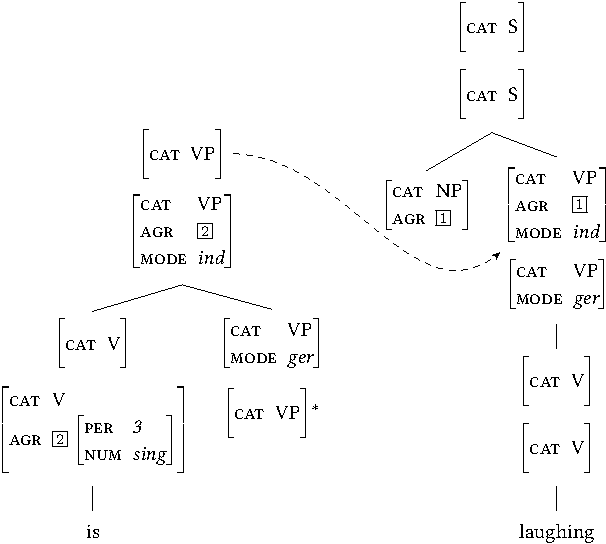
\includegraphics{Figures/tag-obl-adj-ftag-cropped}
}
% This does not work with texlive 2015 use texlive 2013
%% \hfill
%% \begin{forest}
%% [{\subnode{vpone}{\ms{
%%    cat & {\upshape VP}\\
%%  }}\vspace{2mm}\\ 
%%  \ms{
%%        cat & {\upshape VP}\\
%%        agr & \ibox{2}\\ 
%%        mode & ind\\
%%  }}
%%   [{\ms{
%%        cat & {\upshape V}\\
%%       }\vspace{2mm}\\
%%     \ms{
%%       cat & {\upshape V}\\
%%       agr & \ibox{2} \ms{
%%                       per & 3\\ 
%%                       num & sing\\
%%                      }\\
%%        }} [is]]
%%   [{\ms{
%%        cat & {\upshape VP}\\ 
%%        mode & ger\\
%%       }\vspace{2mm}\\
%%     \ms{
%%        cat & {\upshape VP}\\
%%        }$^*$}]]
%% \end{forest}
%% %% %%% sings tree:
%% %% \hspace{-1em}
%% \hfill
%% \begin{forest}
%% [{\ms{ 
%%    cat & {\upshape S}\\
%%  }\vspace{2mm}\\
%%  \ms{
%%   cat & {\upshape S}\\ 
%%   }}
%%   [\ms{ cat & {\upshape NP}\\
%%         agr & \ibox{1}\\
%%       }]
%%   [{\subnode{vptwo}{\ms{
%%       cat  & {\upshape VP}\\
%%       agr  & \ibox{1}\\
%%       mode & ind\\
%%       }}\vspace{2mm}\\
%%      \ms{
%%      cat & {\upshape VP}\\ 
%%      mode & ger\\
%%      }}
%%      [{\ms{ cat & {\upshape V}\\
%%           }\vspace{2mm}\\
%%        \ms{
%%             cat & {\upshape V}\\
%%         }}
%%        [laughing]]]]
%% \end{forest}
%% \hfill\mbox{}
%% \begin{tikzpicture}[overlay,remember picture,out=0,in=220]
%% \draw[->, dashed] (vpone) to (vptwo);
%% \end{tikzpicture}
\caption{\label{Obl-Adjunktion-FTAG}Obligatory adjunction in FTAG}
\end{figure}%
In order for this subtree to be used in a complete structure, another tree has to be added so that
the two parts of the VP node are separated. This happens
by means of an auxiliary tree as shown in Figure~\ref{Obl-Adjunktion-FTAG}. The highest VP node of the auxiliary tree is unified with the upper
VP node of \emph{laughing}. The node of the auxiliary tree marked with `*' is unified with the lower VP node of \emph{laughing}.
The result of this is given in Figure~\vref{Obl-Adjunktion-FTAG-Ergebnis}.
\begin{figure}
%%% is laughing tree:
\centerline{%
\begin{forest}
[{\ms{ 
   cat & {\upshape S}\\
 }\vspace{1mm}\\
  \ms{
   cat & {\upshape S}\\
  }}
  [{\ms{ cat & {\upshape NP}\\
         agr & \ibox{1}\\
   }}]
  [{\ms{
     cat  & {\upshape VP}\\
     agr  & \ibox{1}\\
     mode & ind\\
    }\vspace{1mm}\\
    \ms{
       cat & {\upshape VP}\\
       agr & \ibox{2}\\ 
       mode & ind\\
    }}
    [{\ms{
       cat & {\upshape V}\\
      }\vspace{1mm}\\
      \ms{
        cat & {\upshape V}\\
        agr & \ibox{2} \ms{
                per & 3\\ 
                num & sing\\
               }\\
         }} [is]]
     [{\ms{
        cat & {\upshape VP}\\ 
        mode & ger\\
      }\vspace{1mm}\\
      \ms{
       cat & {\upshape VP}\\ 
       mode & ger\\
      }}
      [{\ms{ cat & {\upshape V}\\
           }\vspace{1mm}\\
        \ms{
             cat & {\upshape V}\\
        }} [laughing]]]]]
\end{forest}
}
\caption{\label{Obl-Adjunktion-FTAG-Ergebnis}Result of obligatory adjunction in FTAG}
\end{figure}%

If a tree is used as a final derivation, the top structures are identified with the bottom structures. Thus, the \textsc{agr} value
of the highest VP node is identified with that of the lower one in the tree in Figure~\ref{Obl-Adjunktion-FTAG-Ergebnis}.
As such, only NPs that have the same \textsc{agr} value as the auxiliary can be inserted into the NP slot.

\addlines
This example shows that, instead of the marking for obligatory adjunction\is{adjunction!obligatory|)} that we saw in the section on long"=distance
dependencies, the same effect can be achieved by using incompatible feature specifications on the top and bottom structures.
If there are incompatible top and bottom structures in a tree, then it cannot be a final derivation
tree and therefore this means that at least one adjunction operation must still take place in order
to yield a well"=formed tree.\is{Tree Adjoining Grammar (TAG)!Feature Structure"=Based (FTAG)|)}

\subsection{V"=TAG}
\label{sec-vtag}

V"=TAG\is{Tree Adjoining Grammar (TAG)!Vector (V-TAG)|(} 
is a variant of TAG proposed by Owen \citet{Rambow94a} that also assumes feature structures on
nodes. In addition, like MC"=TAG, it assumes that elementary trees consist of multiple components. Figure~\vref{Abbildung-Lexical-Set-geben-V-TAG} shows the elementary lexical set
for the ditransitive verb \emph{geben} `give'.
\begin{figure}
\vspace{4\baselineskip}
\menge{ 
\forestset{begin draw/.code={\begin{tikzpicture}[baseline=(current bounding box.center)]}}
    \hspace{1em}
    \begin{forest}
    [, phantom, for children={if n'=1{before computing xy={s*=1.25}}{}}
       %% This adjusts the relative position of the last child by zeroing its distance from the
       %% phantom root and increasing its distance from its sibling. This is delayed because 
       %% otherwise Forest will undo any changes when packing the tree.
      [VP
            [NP$\downarrow$]
            [VP, tikz+={\ignoreme\draw [densely dashed] ([yshift=2.5pt].south) [out=-75, in=-125] to ($(!u.north)!3/4!(!un.north)$) [out=55,in=100] to (!rl.north); }]]
    [VP
            [NP$\downarrow$]
            [VP, tikz+={\ignoreme\draw [densely dashed] ([yshift=2.5pt].south) [out=-75, in=-125] to ($(!u.north)!3/4!(!un.north)$) [out=55,in=100] to (!rl.north); }]]
    [VP
            [NP$\downarrow$]
            [VP, tikz+={\ignoreme\draw [densely dashed] ([yshift=2.5pt].south) [out=-75, in=-125] to ($(!u.north)!3/4!(!un.north)$) [out=55,in=100] to (!rl.north); }]]
    [VP
            [geben]
            [VP, tikz+={\ignoreme\draw [densely dashed] ([yshift=2.5pt].south) [out=-75, in=-125] to ($(!u.north)!3/4!(!un.north)$) [out=55,in=100] to (!rl.north); }]]
    [VP
            [$\epsilon$]]]
    \end{forest}
    \hspace{1em}
}
\vspace{.4\baselineskip}
\caption{\label{Abbildung-Lexical-Set-geben-V-TAG}Lexicon set for \emph{geben} `to give' in V"=TAG
  according to \citet[\page 6]{Rambow94a}}
\end{figure}%
%\addlines
The lexicon set consists of a tree for the verb, an empty element of the category VP and three trees where a VP has been combined with
an NP. As in MC"=TAG, dominance relations are also indicated. The dominance constraints in Figure~\ref{Abbildung-Lexical-Set-geben-V-TAG}
ensure that all lower VP nodes dominate the highest VP node of the tree further to the right. The order of the arguments of the verb as
well as the position of the verb is not given. The only thing required is that lower VP in the NP
trees and lower VP in the \emph{geben} tree dominate the empty VP node.
With this lexicon set, it is possible to derive all permutations of the arguments. Rambow also shows
how such lexical entries can be used to analyze sentences with verbal complexes. Figure~\vref{Abbildung-zu-reparieren-versprochen-V-TAG} shows a verbal complex formed from
\emph{zu reparieren} `to repair' and \emph{versprochen} `promised' and the relevant dominance constraints.
\begin{figure}
\vspace{4\baselineskip}
\oneline{%
\menge{%
  \begin{forest}
    [, phantom, for children={if n'=1{before computing xy={l=0pt, s*=1.25}}{}}
       %% This adjusts the relative position of the last child (n'=1) by zeroing its distance from the
       %% phantom root (l=0) and increasing its distance from its sibling. This is delayed because 
       %% otherwise Forest will undo any changes when packing the tree.
      [VP
        [NP$\downarrow$]
        [VP, tikz+={\ignoreme\draw [densely dashed] ([yshift=2.5pt].south) [out=-75, in=-125] to
            ($(!u.north)!3/4!(!un.north)$) %[out=55,in=181]  to ++(4cm,2cm) [out=-1,in=90] 
            [out=55,in=90] to (!rll.north); }]
        % the following line is ignored for space computation due to \ignoreme
        % the first VP node at the baseline is connected to a place between the dominating vp !u.north and the node to the
        % left of it !un.north (the second VP node on the second line). 3/4 specifies the position
        % between these nodes. It is more to the second VP. From there we go to rll, which is the
        % root node's (r) last child's (l) last child (l). Since the root node is our phantom node,
        % the rll node is the last VP in the second row.
        %
        % the yshift raises the beginning of the line so that it is not too far away from the node.
      ]
      [VP
        [NP$\downarrow$]
        [VP, tikz+={\draw [densely dashed] ([yshift=2.5pt].south) [out=-80, in=180] to ++(20mm,-15mm) [out=0, in=-90] to ($(!unn.north)!.7!(!unnn1.north)$) [out=90, in=180] to ++(3.5mm,5mm) [out=0, in=90] to (!rl1.north); }]
      ]
      [VP
        [NP$\downarrow$]
        [VP, tikz+={\draw [densely dashed] ([yshift=2.5pt].south) [out=-80, in=180] to ++(10mm,-10mm) [out=0, in=-90] to ($(!un.north)!.6!(!unn1.north)$) [out=90, in=180] to ++(5.5mm,6.5mm) [out=0, in=90] to (!rl1.north); }]
      ]
      [VP
        [NP$\downarrow$]
        [VP, tikz+={\draw [densely dashed] ([yshift=2.5pt].south) [out=-80, in=-105] to ($(!u.north)!1/3!(!un.north)$) [out=75,in=90] to (!rll.north); }]
      ]
      [VP
        [VP
          [$\epsilon$]
          [zu reparieren]
        ]
        [VP, baseline
          [$\epsilon$]
          [versprochen]
        ]
      ]
    ]
  \end{forest}
}
}
\vspace{2.5\baselineskip}
\caption{\label{Abbildung-zu-reparieren-versprochen-V-TAG}Analysis of the verbal complex \emph{zu reparieren versprochen} in V"=TAG}
\end{figure}%%
Both of the first NP trees have to dominate \emph{versprochen} and the third and fourth NP tree have to dominate \emph{zu reparieren}.
The order of the NP trees is not restricted and thus all permutations of NPs can be derived.

The interesting thing here is that this approach is similar to the one proposed by \citet[Section~2.1.3]{Berman96a-u} in LFG\indexlfg
(see Section~\ref{Abschnitt-LFG-Umstellung}): in Berman's analysis, the verb projects directly to form a VP and the arguments are
then adjoined. 

A difference to other analyses discussed in this book is that there is always an empty
element\is{empty element} in the derived trees regardless
of verb position.%
\is{Tree Adjoining Grammar (TAG)!Vector (V-TAG)|)}

\subsection{The competence"=performance distinction and the generative capacity of tree"=local MC"=LTAG}
\label{Abschnitt-Kompetenz-Performanz-TAG}

In\is{competence|(}\is{performance|(} many of the theories discussed in this book, a distinction is made between competence and performance
\citep[Section~I.1]{Chomsky65a}. Competence theories are supposed to describe linguistic knowledge, whereas a performance theory should
explain how linguistic knowledge is used and why we make mistakes during speech production and
comprehension, etc. See Chapter~\ref{chap-competence-performance} for further discussion.

\citet*{JBR2000a} discuss examples of center self embedding of relative clauses as those in (\mex{1}b),
and follow \citet[\page 286]{CM63a}  in the assumption that the fact that this kind of embedding is only possible up to three levels should not be
described by grammar, but is rather due to processing problems with the hearer independent of their principle abilities with regard to grammar.
\eal
\label{TAG-Beispiel-Performanz}
\ex 
\gll dass der Hund bellt, der  die Katze jagt,  die  die Maus  gefangen hat\\
     that the dog  barks  that the cat   chases that the mouse caught   has\\
\glt `that the dog that chases the cat that caught the mouse barks'
\ex 
\gll dass der Hund, [$_1$ der  die Katze, [$_2$ die  die Maus  gefangen hat,~$_2$] jagt~$_1$] bellt\\
     that the dog   {}    that the cat    {}    that the mouse caught   has        chases    barks\\
\zl

\noindent
What is interesting in this context is that it is possible to construct examples of center embedding so that they are easier to process
for the hearer. In this way, it is possible to increase the number of center embeddings possible to
process by one and therefore to show that all grammars that formulate a restriction that there may
be at most two center"=embedded relative clauses are incorrect.
The following example from Hans Uszkoreit\ia{Hans Uszkoreit} is easier to process since all embedded relative clauses are isolated and the verbs
are separated by material from the higher clause.
\ea
\gll Die Bänke, [$_1$ auf denen damals die Alten des Dorfes, [$_2$ die allen Kindern, [$_3$ die vorbeikamen $_3$], freundliche Blicke zuwarfen $_2$], 
lange Stunden schweigend nebeneinander saßen $_1$], mussten im letzten Jahr einem~~~~~~~ Parkplatz weichen.\\
the benches {} on which back.then the old.people of.the village {} that all children {} that came.by {} friendly glances gave {}
long hours silent next.to.each.other sat {} must in.the last year a car.park give.way.to\\
\glt `The benches on which the older residents of the village, who used to give friendly glances to all the children who came by, used to sit silently next to one 
another had to give way to a car park last year.'
\z
For other factors that play a role in processing, see \citew{Gibson98a}.

%\addlines
\citet{JBR2000a} discuss verbal complexes with reordered arguments. The general pattern that they
discuss has the form shown in (\mex{1}):
\ea
$\sigma$(NP$_1$ NP$_2$ \ldots{} NP$_n$) V$_{n}$V$_{n-1}$ \ldots{} V$_{1}$
\z
Here, $\sigma$ stands for any permutation of noun phrases and V$_{1}$ is the finite verb.
The authors investigate the properties of Lexicalized Tree Adjoining Grammar (LTAG) with regard to this
pattern and notice that LTAG cannot analyze the order in (\mex{1}) if the semantics is supposed to
come out correctly.
\ea
NP$_2$ NP$_3$ NP$_1$ V$_{3}$V$_{2}$V$_{1}$
\z
Since (\mex{1}) is possible in German, LTAG is not sufficient to analyze all languages.
\ea
\gll dass ihm$_2$ das Buch$_3$ niemand$_1$ zu lesen$_3$ versprechen$_2$ darf$_1$\\
     that him     the book     nobody     to read      promise         be.allowed.to\\
\glt `that nobody is allowed to promise him to read the book' 
\z
Therefore, they propose the extension of TAG discussed in Section~\ref{Abschnitt-MC-TAG}; so"=called
\emph{tree"=local multi"=component LTAG} (Tree"=local MC"=LTAG or TL-MCTAG).
They show that TL-MCTAG can analyze (\mex{0}) but not (\mex{1}) with the correct semantics. They claim that these orders are not possible in German
and argue that in this case, unlike the relative clause examples, one has both options, that is, the
unavailability of such patterns can be explained as a performance phenomenon or as a
competence phenomenon.
\ea
\label{ex-mc-ltag-fails}
NP$_2$ NP$_4$ NP$_3$ NP$_1$ V$_{4}$V$_{3}$V$_{2}$V$_{1}$
\z
If we treat this as a performance phenomenon, then we are making reference to the complexity of the construction and the resulting processing problems
for the hearer. The fact that these orders do not occur in corpora can be explained with reference to the principle of cooperativeness\is{cooperativeness}.
Speakers normally want to be understood and therefore formulate their sentences in such a way that the hearer can understand them.
Verbal complexes in German with more than four verbs are hardly ever found since it is possible to simplify very complex sentences with multiple verbs in the 
right sentence bracket by extraposing\is{extraposition} material and therefore avoiding ambiguity\is{ambiguity} (see \citealp[\page 5]{Netter91} and
\citealp[\page 262]{MuellerLehrbuch1}).

The alternative to a performance explanation would involve using a grammatical formalism which is
just powerful enough to allow embedding of two verbs and reordering of their arguments, but rules
out embedding of three verbs and reordering of the arguments. \citet{JBR2000a} opt for this solution
and therefore attribute the impossibility of the order of arguments in (\mex{0}) to competence. 

In HPSG (and also in Categorial Grammar\indexcg and in some GB analyses\indexgb), verbal complexes are analyzed by means of argument composition
\citep{HN89b,HN94a}. Under this approach, a verbal complex behaves exactly like a simplex verb and the arguments of the verbs involved can be placed
in any order. The grammar does not contain any restriction on the number of verbs that can be combined, nor any constraints that ban embedding below a certain
level. In the following, I will show that many reorderings are ruled out by communication rules that
apply even with cases of simple two"=place verbs. The conclusion is that the impossibility of embedding four or more verbs should in fact be explained as a performance issue.

Before I present arguments against a competence"=based exclusion of (\ref{ex-mc-ltag-fails}), I will make a more general comment:
corpora cannot help us here since one does not find any instances of verbs with four or more embeddings. \citet{Bech55a} provides
an extensive collection of material, but had to construct the examples with four embedded verbs.
\citet[\page 94--95]{Meurers99c} gives constructed examples with five verbs that contain multiple auxiliaries or modal verbs.
These examples are barely processable and are not relevant for the discussion here since the verbs in (\ref{ex-mc-ltag-fails})
have to select their own arguments. There are therefore not that many verbs left when constructing examples. It is possible to only use subject
control verbs with an additional object (\eg \emph{versprechen} `to promise'), object control verbs (\eg \emph{zwingen} `to force')
or AcI verbs (\eg \emph{sehen} `to see' or \emph{lassen} `to let') to construct examples.
When constructing examples, it is important make sure that all the nouns involved differ as much as possible with regard to their
case\is{case} and their selectional restrictions\is{selection!restriction} (\eg animate/inanimate) since these are features that a hearer/reader could
use to possibly assign reordered arguments to their heads. If we want to have patterns such as (\ref{ex-mc-ltag-fails}) with four NPs each with a different
case, then we have to choose a verb that governs the genitive.
There are only a very small number of such verbs in German. Although the example constructed by \citet{JBR2000a} in (\ref{Beispiel-Joshi-NP4}) fulfills
these requirements, it is still very marked. It therefore becomes clear that the possibility of finding a corresponding example in a newspaper article
is extremely small. This is due to the fact that there are very few situations in which such an utterance would be imaginable. Additionally,
all control verbs (with the exception of \emph{helfen} `to help') require an infinitive with \emph{zu} `to' and can also be realized incoherently, that is,
with an extraposed infinitival complement without verbal complex formation. As mentioned above, a
cooperative speaker/""author would use a less complex construction and this reduces the probability
that these kinds of sentences arise even further.

Notice that tree"=local MC-LTAG does not constrain the number of verbs in a sentence. The formalism allows for an arbitrary number of verbs.
It is therefore necessary to assume, as in other grammatical theories, that performance constraints are responsible for the fact that we never find
examples of verbal complexes with five or more verbs. Tree"=local MC-LAG makes predictions about the possibility of arguments to be reordered.
I consider it wrong to make constraints regarding mobility of arguments dependent on the power of the grammatical formalism since the restrictions that
one finds are independent of verbal complexes and can be found with simplex verbs taking just two arguments.
The problem with reordering is that it still has to be possible to assign the noun phrases to the
verbs they belong to. If this assignment leads to ambiguity\is{ambiguity}
that cannot be resolved by case, selectional restrictions, contextual knowledge or intonation, then the unmarked constituent order is chosen.
\citet*[\page 68]{Hoberg81a} shows this very nicely with examples similar to the
following:\footnote{%
 Instead of \emph{das} `the', Hoberg uses the possessive pronoun \emph{ihr} `her'.
 This makes the sentences more semantically plausible, but one then gets interference from the
 linearization requirements for bound pronouns. I have therefore replaced the pronouns with the
 definite article.%
}
\eal
\judgewidth{\#}
\ex[]{
\gll Hanna hat immer schon gewußt, daß das Kind sie verlassen will.\\
	 Hanna has always already known that the child she leave wants\\
\glt `Hanna has always known that the child wants to leave her.'
}
\ex[\#]{
\gll Hanna hat immer schon gewußt, daß sie das Kind verlassen will.\\
     Hanna has always already known that she the child  leave wants\\
\glt Preferred reading: `Hanna has always known that she wants to leave the child.'
}
\ex[]{
  \raggedright
\gll Hanna hat immer schon gewußt, daß sie der Mann verlassen will.\\
     Hanna has always already known that she the.\nom{} man leave wants.to\\
\glt `Hanna has always known that the man wants to leave her.'
}
\zl
%\pagebreak

\noindent
It is not possible to reorder (\mex{0}a)  to (\mex{0}b) without creating a strong preference for another reading.
This is due to the fact that neither \emph{sie} `she' nor \emph{das Kind} `the child' are unambiguously marked as
nominative or accusative. (\mex{0}b) therefore has to be interpreted as Hanna being the one that wants something, namely
to leave the child. This reordering is possible, however, if at least one of the arguments is unambiguously marked for case
as in (\mex{0}c).

For noun phrases with feminine count nouns, the forms for nominative and accusative as well as genitive and dative are the same.
For mass nouns, it is even worse. If they are used without an article, all cases are the same for feminine nouns (\eg \emph{Milch} `milk')
and also for masculines and neuters with exception of the genitive. In the following example from
\citet[\page 45]{Wegener85b} it is hardly possible to switch the dative and accusative object,
whereas this is possible if the nouns are used with articles as in (\mex{1}c,d): 

\eal
\ex 
\gll Sie mischt Wein Wasser bei.\\
     she mixes wine water into\\
\glt `She mixes water into the wine.'
\ex 
\gll Sie mischt Wasser Wein bei.\\
     she mixes water wine into\\
\glt `She mixes wine into the water.'
\ex 
\gll Sie mischt dem Wein das Wasser bei.\\
     she mixes the.\dat{} wine the.\acc{} water into\\
\glt `She mixes the water into the wine.'
\ex 
\gll Sie mischt das Wasser dem Wein bei.\\
	she mixes the.\acc{} water the.\dat{} wine into\\
\glt `She mixes the water into the wine.'
\zl
The two nouns can only be switched if the meaning of the sentence is clear from the context (\eg through explicit negation of the opposite)
and if the sentence carries a certain intonation.

The problem with verbal complexes is now that with four noun phrases, two of them almost always have the same case if one does not wish to
resort to the few verbs governing the genitive. A not particularly nice-sounding example of morphologically unambiguously marked case
is (\mex{1}):
\ea
\gll weil    er        den        Mann dem        Jungen des Freundes gedenken helfen lassen will\\
     because he.\nom{} the.\acc{} man  the.\dat{} boy    of.the.\gen{} friend remember help let wants\\
\glt `because he wants to let the man help the boy remember his friend'
\z
Another strategy is to choose verbs that select animate and inanimate objects so that animacy of the arguments can aid interpretation.
I have constructed such an example where the most deeply embedded predicate is not a verb but rather an adjective. The predicate \emph{leer fischen}
`to fish empty' is a resultative construction that should be analyzed parallel to verbal complexes \citep[Chapter~5]{Mueller2002b}.
\ea
\gll weil niemand$_1$ [den Mann]$_2$ [der Frau]$_3$ [diesen Teich]$_4$  leer$_4$ fischen$_3$ helfen$_2$ sah$_1$\\
     because nobody.\nom{} \spacebr{}the.\acc{} man \spacebr{}the.\dat{} woman \spacebr{}this.\acc{} pond empty fish help saw\\
\glt `because nobody saw the man help the woman fish the pond empty'
\z
If one reads the sentences with the relevant pauses, it is comprehensible. Case is unambiguously marked on the animate
noun phrases and our word knowledge helps us to interpret \emph{diesen Teich} `this pond' as the argument of \emph{leer} `empty'.  

\largerpage[-1]
The sentence in (\mex{0}) would correctly be analyzed by an appropriately written tree"=local MC-LTAG and also by argument composition
analyses for verbal complexes and resultative constructions. The sentence in (\mex{1}) is a variant of (\mex{0}) that corresponds exactly
to the pattern of (\ref{ex-mc-ltag-fails}):
\ea
\gll weil [der Frau]$_2$ [diesen Teich]$_4$ [den Mann]$_3$ niemand$_1$ leer$_4$ fischen$_3$ helfen$_2$ sah$_1$\\
	 because \spacebr{}the.\dat{} woman \spacebr{}this.\acc{} pond \spacebr{}the.\acc{} man nobody.\nom{} empty fish help saw\\
\glt `because nobody saw the man help the woman fish the pond empty'
\z
(\mex{0}) is more marked than (\mex{-1}), but this is always the case with local reordering (Gisbert Fanselow\ia{Gisbert Fanselow}, p.\,c.\ 2006).
This sentence should not be ruled out by the grammar. Its markedness is more due to the same factors that were responsible for the markedness of reordering
of arguments of simplex verbs. Tree"=local MC-LTAG can not correctly analyze sentences such as (\mex{0}), which shows that this TAG variant is not
sufficient for analyzing natural language.

There are varying opinions among TAG researchers as to what should be counted as competence and what
should be counted as performance. For instance, \citet[\page 15]{Rambow94a} argues that one should
not exclude reorderings that cannot be processed by means of competence grammar or the grammatical
formalism. In Chapter~6, he presents a theory of performance that can explain why the reordering of
arguments of various verbs in the middle field is harder to process.
One should therefore opt for TAG variants such as V-TAG\is{Tree Adjoining Grammar (TAG)!Vector (V-TAG)} or TT-MC-TAG\is{Tree Adjoining Grammar (TAG)!Tree Tuple MC-TAG (TT-MC-TAG)} \citep{Lichte2007a} that are powerful enough to analyze the diverse reorderings
	and then also use a performance model that makes it possible to explain the gradual differences in acceptability.

An alternative to looking for a grammatical formalism with minimal expressive power is to not restrict the grammatical formalism at all with regard
to its expressive power and instead develop as restrictive linguistic theories as possible. For further discussion of this point, see 
Chapter~\ref{sec-generative-capacity}.
\is{competence|)}\is{performance|)}

\section{Summary and classification}

\largerpage[-1]
%\enlargethispage{4pt}
In sum, we have seen the following: LTAG is lexicalized, that is, there is at least one lexical element in every tree.
There are not any trees that correspond to the rule S $\to$ NP VP since no words are mentioned in this rule.
Instead, there are always complex trees that contain the subject NP and the VP. Inside the VP, there can be as much structure
as is necessary to ensure that the verb is contained in the tree. As well as the head, elementary trees in LTAG always contain
the arguments of the head. For transitive verbs, this means that both the subject and the object have to be components of the
elementary tree. This is also true of the trees used to analyze long"=distance dependencies. As shown in Figure~\ref{abb-nld-TAG},
the object must be part of the tree. The fact that the object can be separated from the verb by multiple sentence boundaries is not
represented in the elementary tree, that is, recursive\is{recursion} parts of grammar are not contained in elementary trees.
The relevant effects are achieved by adjunction, that is, by insertion of material into elementary trees.
The elementary tree for extraction in Figure~\ref{abb-nld-TAG} differs from the elementary tree for \emph{likes} given in
Figure~\ref{Abbildung-Max-likes-Anouk} for the use in normal SVO clauses. Every minimal construction, in which \emph{likes}
can occur (subject extraction, topicalization, subject relative clauses, object relative clauses, passive, \ldots) needs its own
elementary tree \citep[\page 10]{KJ2003a}. The different elementary trees can be connected using lexical rules\is{lexical rule}.
These lexical rules map a particular tree treated as underlying to other trees. In this way, it is possible to derive
a passive tree from an active tree. These lexical rules are parallel to transformations\is{transformation} in Transformational
Grammar, however, one should bear in mind that there is always a lexical element in the tree, which makes the entire grammar
more restrictive than grammars with free transformations.

An interesting difference to GB and variants of LFG, CG, and HPSG that assume empty elements\is{empty element} is that
the variants of TAG presented here\footnote{%
	See \citew{Rambow94a} and \citew[\page 194]{Kallmeyer2005a-u}, however, for TAG analyses with an empty element in the lexicon.%
} do not contain empty elements in the lexicon. They can be used in trees but trees are listed as a whole in the lexicon.

Elementary trees can be of any size, which makes TAG interesting for the analysis of idioms (see Section~\ref{Abschnitt-Diskussion-Lokalitaet}). 
Since recursion is factored out, trees can contain elements that appear very far away from each other in
the derived tree (extended domains of locality\is{locality}).

\citet*{KKNV95a} show that it is possible to transfer HPSG grammars that fulfill certain requirements into TAG grammars. This is interesting
as in this way one arrives at a grammar whose complexity behavior is known\is{capacity!generative}. Whereas HPSG grammars are generally
in the Type-0 area, TAG grammars can, depending on the variant, fall into the realm of Type-2 languages (context"=free) or even in the
larger set of the mildly context"=sensitive grammars\is{mildly context"=sensitive grammar!context"=sensitive grammar} \citep{Joshi85a-u}. \citet*{YMTT2001a} have developed a procedure for translating FB"=LTAG grammars into
HPSG grammars.


\bigskip
\questions{

\begin{enumerate}
\item How are long"=distance dependencies analyzed in TAG? Does one need empty elements for this?
\item Is it possible to analyze the reordering of arguments of multiple verbs using standard TAG processes?
\end{enumerate} 
}

\exercises{

\begin{enumerate}
\item Analyze the following string in LTAG:
\ea
\gll der dem König treue Diener\\
	 the the.\dat{} king loyal servant\\
\glt `the servant loyal to the king'
\z
\end{enumerate}
}

\furtherreading{

Some important articles are \citew*{JLT75a-u}, \citew{Joshi87a-u}, and \citew{JS97a}. Many works discuss formal properties of TAG and are therefore not particularly accessible for
linguistically interested readers. \citew{KJ85a} give a good overview of linguistic analyses. An overview of linguistic and computational linguistic
works in TAG can be found in the volume edited by Abeill{\'e} and
Rambow\nocite{AR2000a-ed-not-crossreferenced} from 2000. \citet{Rambow94a} compares his TAG variant (V"=TAG\is{Tree
  Adjoining Grammar (TAG)!Vector (V-TAG)}) to Karttunen's \emph{Radical Lexicalism} approach, Uszkoreit's GPSG\indexgpsg,
Combinatorial Categorial Grammar\indexcg, HPSG\indexhpsg and
Dependency Grammar\indexdg. 

\citet{SJ93a} discuss psycholinguistically plausible processing models and show that it is possible to do incremental parsing with TAG. They also present a
further variant of TAG: synchronous TAG\indexstag. In this TAG variant, there is a syntactic tree and a semantic tree connected to it.
When building syntactic structure, the semantic structure is always built in parallel. This structure built in parallel corresponds to the level of Logical
Form\is{Logical Form (LF)} derived from S"=Structure\is{S"=Structure} using transformations\is{transformation} in GB.


\citet[Chapter~6]{Rambow94a} presents an automaton"=based performance theory. He applies it to German and shows that
the processing difficulties that arise when reordering arguments of multiple verbs can be explained.
\is{Tree Adjoining Grammar (TAG)|)}

\citet{KR2008a-u} show how it is possible to derive MRS representations directly via a derivation tree using FTAG. In each top node, there is a reference
to the semantic content of the entire structure and each bottom node makes reference to the semantic content below the node. In this way, it becomes possible
to insert an adjective (\eg \emph{mutmaßlichen} `suspected') into an NP tree \emph{alle Mörder} `all murderers' so that the adjective has scope over
the nominal part of the NP (\emph{Mörder} `murderers'): for adjunction of the adjective to the N node, the adjective can access the semantic content of the noun.
The top node of \emph{mutmaßlichen} is then the top node of the combination \emph{mutmaßlichen Mörder} `suspected murderers' and this ensures that the meaning of \emph{mutmaßlichen Mörder}
is correctly embedded under the universal quantifier.}


%      <!-- Local IspellDict: en_US-w_accents -->
